\documentclass{article}

\usepackage{fancyhdr}
\usepackage{extramarks}
\usepackage{amsmath}
\usepackage{amsthm}
\usepackage{amsfonts}
\usepackage{tikz}
\usepackage[plain]{algorithm}
\usepackage{algpseudocode}
\usepackage{enumitem}
\usepackage{mathtools}
\usepackage{amssymb}
\usetikzlibrary{automata,positioning}
\usepackage{pgfplots}
\usepackage{graphicx}


%
% Basic Document Settings
%

\topmargin=-0.45in
\evensidemargin=0in
\oddsidemargin=0in
\textwidth=6.5in
\textheight=9.0in
\headsep=0.25in

\linespread{1.1}

\pagestyle{fancy}
\lhead{\hmwkClass\ \hmwkTitle}
\rhead{\hmwkAuthorName}
\lfoot{\lastxmark}
\cfoot{\thepage}

\renewcommand\headrulewidth{0.4pt}
\renewcommand\footrulewidth{0.4pt}

\setlength\parindent{0pt}

%
% Added stuff
%

\DeclarePairedDelimiter\abs{\lvert}{\rvert}
\setenumerate[0]{label={(\alph*)}}

\pgfplotsset{my style/.append style={axis x line=middle, axis y line=
           middle, xlabel={$x$}, ylabel={$y$}, axis equal }}

%
% Create Problem Sections
%

\newcommand{\enterProblemHeader}[1]{
    \nobreak\extramarks{}{Problem \arabic{#1} continued on next page\ldots}\nobreak{}
    \nobreak\extramarks{Problem \arabic{#1} (continued)}{Problem \arabic{#1} continued on next page\ldots}\nobreak{}
}

\newcommand{\exitProblemHeader}[1]{
    \nobreak\extramarks{Problem \arabic{#1} (continued)}{Problem \arabic{#1} continued on next page\ldots}\nobreak{}
    \stepcounter{#1}
    \nobreak\extramarks{Problem \arabic{#1}}{}\nobreak{}
}

\setcounter{secnumdepth}{0}
\newcounter{partCounter}
\newcounter{homeworkProblemCounter}
\setcounter{homeworkProblemCounter}{1}
\nobreak\extramarks{Problem \arabic{homeworkProblemCounter}}{}\nobreak{}

%
% Homework Problem Environment
%
% This environment takes an optional argument. When given, it will adjust the
% problem counter. This is useful for when the problems given for your
% assignment aren't sequential. See the last 3 problems of this template for an
% example.
%
\newenvironment{homeworkProblem}[1][-1]{
    \ifnum#1>0
        \setcounter{homeworkProblemCounter}{#1}
    \fi
    \section{Problem \arabic{homeworkProblemCounter}}
    \setcounter{partCounter}{1}
    \enterProblemHeader{homeworkProblemCounter}
}{
    \exitProblemHeader{homeworkProblemCounter}
}

%
% Homework Details
%   - Title
%   - Due date
%   - Class
%   - Section/Time
%   - Instructor
%   - Author
%

\newcommand{\hmwkTitle}{Final Exam}
\newcommand{\hmwkDueDate}{March 21, 2017}
\newcommand{\hmwkClass}{DSE 210}
\newcommand{\hmwkClassTime}{}
\newcommand{\hmwkClassInstructor}{Professor: A. Enis \c{C}etin}
\newcommand{\hmwkClassTA}{Teaching Assistant: Shivani Agrawal}
\newcommand{\hmwkAuthorName}{\textbf{Joshua Wilson} \and \textbf{A53228518}}

%
% Title Page
%

\title{
    \vspace{2in}
    \textmd{\textbf{\hmwkClass:\ \hmwkTitle}}\\
    \vspace{0.1in}\large{\textit{\hmwkClassInstructor}}\\
    \vspace{0.1in}\large{\textit{\hmwkClassTA}}
    \vspace{3in}
}

\author{\hmwkAuthorName}
\date{}

\renewcommand{\part}[1]{\textbf{\large Part \Alph{partCounter}}\stepcounter{partCounter}\\}

%
% Various Helper Commands
%

% Useful for algorithms
\newcommand{\alg}[1]{\textsc{\bfseries \footnotesize #1}}

% For derivatives
\newcommand{\deriv}[1]{\frac{\mathrm{d}}{\mathrm{d}x} (#1)}

% For partial derivatives
\newcommand{\pderiv}[2]{\frac{\partial}{\partial #1} (#2)}

% Integral dx
\newcommand{\dx}{\mathrm{d}x}

% Alias for the Solution section header
\newcommand{\solution}{\textbf{\large Solution}}

% Probability commands
\newcommand{\E}{\mathrm{E}}
\newcommand{\Var}{\mathrm{Var}}
\newcommand{\Cov}{\mathrm{Cov}}
\newcommand{\Bias}{\mathrm{Bias}}
\newcommand*{\Perm}[2]{{}_{#1}\!P_{#2}}%
\newcommand*{\Comb}[2]{{}_{#1}C_{#2}}%
\newcommand\given[1][]{\:#1\vert\:}
\newcommand{\norm}[1]{\left\lVert#1\right\rVert}
\DeclareMathOperator*{\argmax}{arg\,max}

\begin{document}

\maketitle

\pagebreak


\begin{homeworkProblem}[1]
$Given:$  \\
Urn A contains 2 white balls and 4 red balls; \\
Urn B contains 8 white balls and 5 red balls; \\
Urn C contains 1 white ball and 3 red balls. \\
$p(Urn\ A) = 0.5$, and $p(Urn\ B) = p(Urn\ C)$

\begin{enumerate}
\item
$p(Urn\ A \given red) = \cfrac{p(red \given Urn\ A) \times p(Urn\ A)}{p(red)} = \cfrac{\frac{4}{6} \times \frac{1}{2}}{p(red)}$, and \\ \\
$\begin{aligned}
p(red) &= p(red \given Urn\ A) \times p(Urn\ A) + p(red \given Urn\ B) \times p(Urn\ B) + p(red \given Urn\ C) \times p(Urn\ C) \\
&= \bigg( \frac{4}{6} \bigg) \bigg( \frac{1}{2} \bigg) + \bigg( \frac{5}{13} \bigg) \bigg( \frac{1}{4} \bigg) + \bigg( \frac{3}{4} \bigg) \bigg( \frac{1}{4} \bigg) \\
&= \bigg( \frac{4}{12} \bigg) + \bigg( \frac{5}{52} \bigg) + \bigg( \frac{3}{16} \bigg) = \frac{208 + 60 + 117}{624} = \frac{385}{624} \approx 0.617\text{, so}
\end{aligned}$ \\ \\
$p(Urn\ A \given red) = \cfrac{\frac{4}{6} \times \frac{1}{2}}{\frac{385}{624}} = \cfrac{\frac{4}{12}}{\frac{385}{624}} = \boxed{\frac{208}{385} \approx 0.54}$
\item
$p(white) = 1 - p(red) = 1 - \cfrac{385}{624} = \boxed{\cfrac{239}{624} \approx 0.38}$
\end{enumerate}
\end{homeworkProblem}


\begin{homeworkProblem}[2]
Let set $X = \{x_1, x_2, \ldots, x_n\}$.
\begin{enumerate}
\item
We can create a subset of $X$ by choosing any k elements of $X$, such that there are $\binom{n}{k}$ possible subsets of size k.  There are therefore $\sum_{k=0}^{n} \binom{n}{k}$ total subsets of $X$.  \\ \\
By applying the binomial theorem, we have
\begin{equation*}
\sum_{k=0}^{n} \binom{n}{k} = \sum_{k=0}^{n} \binom{n}{k} 1^{n-k} 1^k = (1 + 1)^n = 2^n
\end{equation*}
Alternatively, every element $x_i \in X$ will either be included or excluded from a subset of $X$, and we can create a subset of $X$ by either including or excluding each $x_i$, and the choice of including or excluding each $x_i$ is independent. \\ \\
Since we have 2 choices for n elements, there are $2^n$ possible subsets of $X$ that we can create.
\item
Since there are $2^n$ total subsets of $X$ as shown in part (a), and one is the empty set $\varnothing$, there are $2^n - 1$ nonempty subsets of $X$.  We will construct all nonempty subsets of $X$ as follows:
\begin{enumerate}[label=Step \arabic*:]
\item
Take element $x_1$, and create the union of $x_1$ with every possible subset of the n-1 elements in $\{x_2, x_3, \ldots, x_n\}$. As shown in part (a), the number of subsets of $\{x_2, x_3, \ldots, x_n\}$ is $2^{n-1}$.  Because we are adding $x_1$ to each of these subsets, none will be empty, and they will all include the element $x_1$.
\item
Take element $x_2$, and create the union of $x_2$ with every possible subset of the n-2 elements in $\{x_3, x_4, \ldots, x_n\}$.  We will have $2^{n-2}$ nonempty subsets of $X$, each of which includes element $x_2$, and none of which include element $x_1$.  Thus, we have created $2^{n-2}$ new subsets of $X$.
\item[\vdots\ \ \ \ ]
\item[Step k:]
Take element $x_k$, and create the union of $x_k$ with every possible subset of the n-k elements in $\{x_{k+1}, x_{k+2}, \ldots, x_n\}$.  We will have $2^{n-k}$ nonempty subsets of $X$, each of which includes element $x_k$, and none of which include elements in $\{x_1, x_2, \ldots, x_{k-1}\}$.  Thus, we have created $2^{n-k}$ new subsets of $X$.
\item[\vdots\ \ \ \ ]
\item[Step n:]
Take element $x_n$, and create the union of $x_n$ with the empty set $\varnothing$.  We will have a single nonempty subset of $X$ (i.e. $\{x_n\}$), which includes no elements in $\{x_1, x_2, \ldots, x_{n-1}\}$.  Thus, we have created $1 = 2^0$ new subset of $X$.
\end{enumerate}
At each step $k$ above, we created $2^{n-k}$ unique, nonempty subsets of $X$.  The total number of nonempty subsets of $X$ is therefore $\sum_{k=1}^{n} 2^{n-k}$, so $2^n - 1 = \sum_{k=1}^{n} 2^{n-k}$.
\end{enumerate}
\end{homeworkProblem}


\begin{homeworkProblem}[3]
$Given: \\
p(X = 1) = 0.5$ \\
$p(X = 2) = 0.25$ \\
$p(X = 3) = 0.25$
\begin{enumerate}
\item
$\mathbb{E}[X] = \sum_{x} x \times p(X = x) = 1 \times 0.5 + 2 \times 0.25 + 3 \times 0.25 = 0.5 + 0.5 + 0.75 = \boxed{1.75}$
\item
\begin{align*}
var[X] &= \mathbb{E}[X^2] - \mathbb{E}[X]^2, \text{ and} \\
\mathbb{E}[X^2] &= 1^2 \times 0.5 + 2^2 \times 0.25 + 3^2 \times 0.25 = 0.5 + 4 \times 0.25 + 9 \times 0.25 = 0.5 + 1 + 2.25 = 3.75, \text{ and} \\
\mathbb{E}[X]^2 &= 1.75^2 = 3.0625 \text{, so} \\
var[X] &= 3.75 - 3.0625 = \boxed{0.6875}
\end{align*}
\item
\ \\
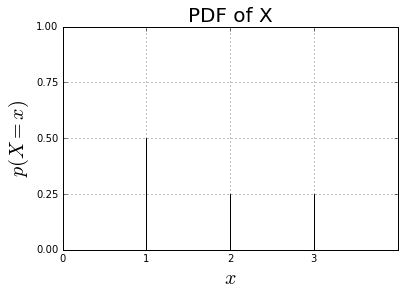
\includegraphics[scale=0.5]{DSE210_Q3_c_pdf}
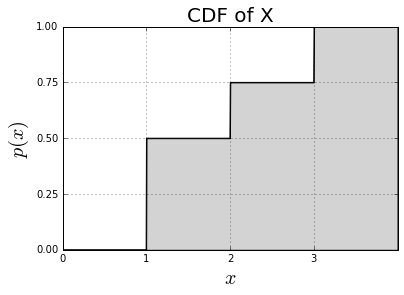
\includegraphics[scale=0.5]{DSE210_Q3_c_cdf}

\end{enumerate}
\end{homeworkProblem}

\newpage
\begin{homeworkProblem}[4]
See DSE210\_Final\_Q4.ipynb notebook at https://github.com/mas-dse/jsw037/tree/master/DSE210.
\begin{enumerate}
\item
Error rate on the test dataset is 0.3767.
\item
Confusion Matrix: \\
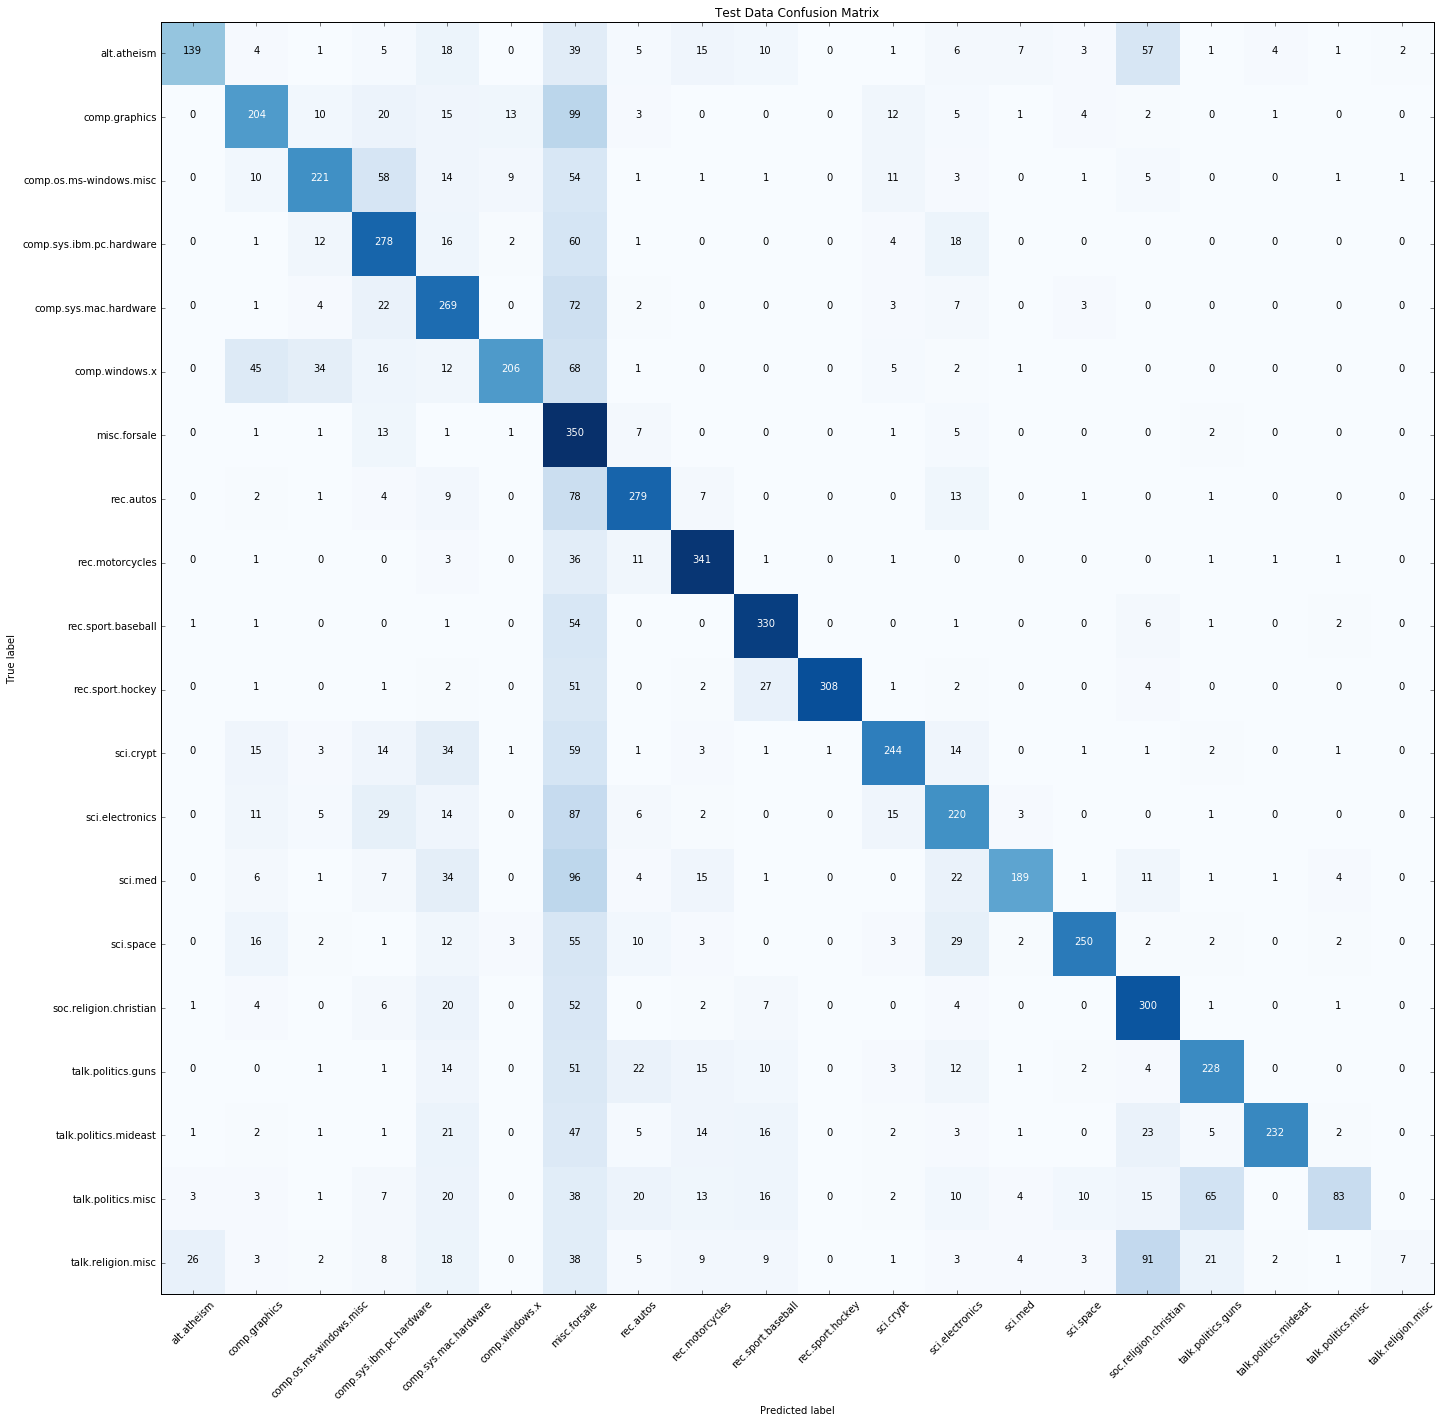
\includegraphics[width=\linewidth]{DSE210_Q4_b}
\end{enumerate}
\end{homeworkProblem}

\newpage
\begin{homeworkProblem}[5]
$Given:  \vec{w} = \begin{bmatrix} -1 \\ 2 \end{bmatrix}, \theta = 10$.  Find the decision boundary $\vec{w} \bullet \vec{x} \geq \theta$ in $\mathbb{R}^2$.\\ \\
Let $\vec{x} = \begin{bmatrix} x \\ y \end{bmatrix}$, then $\vec{w} \bullet \vec{x} = \begin{bmatrix} -1 \\ 2 \end{bmatrix} \bullet \begin{bmatrix} x \\ y \end{bmatrix} = -1 x + 2 y \geq 10 \implies y \geq 5 + \frac{1}{2} x$.  \\ \\
If $x = 0$, then $y \geq 5$, and if $y = 0$, then $x \leq -10$.  \\ \\
The decision boundary is depicted below: \\ \\
\begin{tikzpicture}
         \begin{axis}[my style, minor tick num = 1]
		\addplot[domain=-15:5]{1/2 * x+5};
		\node (b) at (axis cs:-7,4){boundary};
		\node (+) at (axis cs:	-6,3){+};
		\node (-) at (axis cs:-4.5,2){-};
		\node (source) at (axis cs:0,0){};
       		\node (destination) at (axis cs:-1,2){$\vec{w}$};
       		\draw[->](source)--(destination);
    \end{axis}
\end{tikzpicture}


\end{homeworkProblem}


\begin{homeworkProblem}[6]
$Given:$  \\
Urn A $\sim N(0, 1)$, \ \ \ \ $p(A) = \frac{2}{3}$, \ \ \ \ Urn B $\sim N(5, 2)$, \ \ \ \ $p(B) = \frac{1}{3}$
\begin{enumerate}
\item
$p(A \given x = 2.5) = \cfrac{p(x = 2.5 \given A) \times p(A) }{p(x = 2.5)} = \cfrac{p(x = 2.5 \given A) \times p(A) }{p(x = 2.5 \given A) \times p(A)  + p(x = 2.5 \given B) \times p(B)}$, \\ \\
where $p(x = 2.5 \given A) = \cfrac{1}{\sqrt{2 \pi \sigma_A^2}} \text{ exp} \bigg( - \cfrac{(2.5 - \mu_A)^2}{2 \sigma_A^2} \bigg) = \cfrac{1}{\sqrt{2 \pi (1)^2}} \text{ exp} \bigg( - \cfrac{(2.5 - (0))^2}{2 (1)^2} \bigg) \approx 0.01753$, \\ \\
and $p(x = 2.5 \given B) = \cfrac{1}{\sqrt{2 \pi \sigma_B^2}} \text{ exp} \bigg( - \cfrac{(2.5 - \mu_B)^2}{2 \sigma_B^2} \bigg) = \cfrac{1}{\sqrt{2 \pi (2)^2}} \text{ exp} \bigg( - \cfrac{(2.5 - (5))^2}{2 (2)^2} \bigg) \approx 0.09132$, \\ \\
so $p(A \given x = 2.5) \approx \cfrac{(0.01753) \times \frac{2}{3}}{(0.01753) \times \frac{2}{3} + (0.09132) \times \frac{1}{3}} \approx \cfrac{0.01169}{0.04213} = \boxed{0.2774}$
\newpage
\item
Our prediction is based on the higher of $p(A) \times p(x \given A)$ and $p(B) \times p(x \given B)$.  The decision boundary is the point at which $p(A) \times p(x \given A) = p(B) \times p(x \given B)$.  This value is approximately $\boxed{2.181}$. \\ \\
$p(A) \times p(x \given A)$ and $p(B) \times p(x \given B)$ are plotted below in red and blue, respectively, along with the vertical decision boundary line. \\ \\
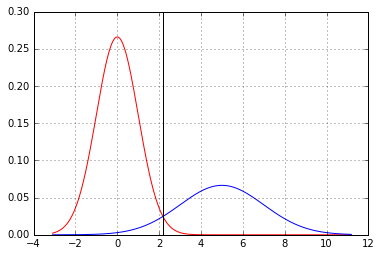
\includegraphics[scale=0.75]{DSE210_Q6_b} \\ \\
See DSE210\_Final\_Scratch.ipynb notebook at https://github.com/mas-dse/jsw037/tree/master/DSE210.
\end{enumerate}
\end{homeworkProblem}


\begin{homeworkProblem}[7]
A histogram of $X = \{\text{-0.1, -0.2, 0.1, 0.2, 0, 0.1, -0.1, 0, -0.05, 0.1, 1.05, 1.1, 0.9, 0.8, 0.9, 1, 1.2, 1.1, 1.2, 0.9}\}$ is below. \\ \\
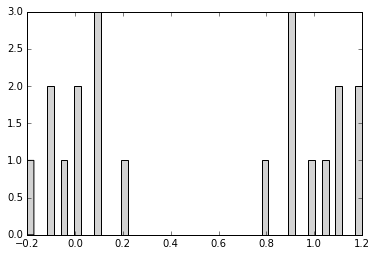
\includegraphics[scale=0.75]{DSE210_Q7} \\ \\
The cluster centers are located at $\boxed{0.005\text{ and }1.015}$. \\ \\
See DSE210\_Final\_Scratch.ipynb notebook at https://github.com/mas-dse/jsw037/tree/master/DSE210.
\end{homeworkProblem}

\begin{homeworkProblem}[8]
The best estimate for the number of mixtures is two:  \\ \\
$N(\mu_1 = 0.005, \sigma_1^2 = 0.014225)$ and $N(\mu_2 = 1.015, \sigma_2^2 = 0.018025)$.  \\ \\
The best estimate was determined by trying from 1 to 10 mixtures and choosing the mixture with the lowest Akaike information criterion and Bayesian information criterion.\\ \\
A plot of the original data and the Gaussians is below: \\ \\
 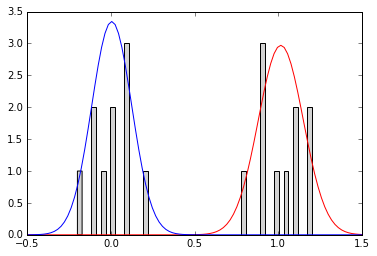
\includegraphics[scale=0.75]{DSE210_Q8} \\ \\
 See DSE210\_Final\_Scratch.ipynb notebook at https://github.com/mas-dse/jsw037/tree/master/DSE210.
\end{homeworkProblem}


\begin{homeworkProblem}[9]
$Given: \\
n = 1000, \ \ \ \text{sample average 307}, \ \ \ \text{sample standard deviation 30},$ \\ \\
The estimate of the nationwide average is $\hat{\mu} = 307$. \\ \\
The standard deviation of this estimate is equal to the sample standard deviation divided by $\sqrt{n}$, so $\hat{\sigma} = \cfrac{30}{\sqrt{1000}} \approx \boxed{0.9487}$.
\end{homeworkProblem}

\newpage
\begin{homeworkProblem}[10]
$Given:$ \\
A random sample of 48 men and 55 women produced the following results: \\ \\
\begin{tabular}{l c c}
							 & Men & Women \\
\hline
Never Married 					 & 43.8\% & 16.4\% \\
Married            					 & 41.7\% & 70.9\% \\
Widowed, divorced, separated           & 14.6\% & 12.7\% \\
							\hline
Total							& 100\% & 100\% \\
\end{tabular} \\ \\

We will test the hypothesis that there is no differences in the distribution of results for men and women by performing a $\chi^2$ test.   \\ \\
Define the null hypothesis as $H_0:$ The results for men and women come from the same distribution. \\ \\
To do so, we estimate the underlying distribution and expected frequencies for each of the two samples by aggregating the results: \\

\begin{tabular}{l c c | c c | c | c}
							 & Men \% & Women \% & Men Obs & Women Obs & Total Obs & Exp \%\\
							 \hline
Never Married 					 & 43.8\% & 16.4\% & 21 & 8 & 30 & 29.1\% \\
Married            					 & 41.7\% & 70.9\% & 20 & 39 & 59 & 57.3\% \\
Widowed, divorced, separated           & 14.6\% & 12.7\% & 7  & 7 & 14 & 13.6\% \\
							\hline
Total							& 100\% & 100\% & 48 & 55 & 103 & 100\% \\
\end{tabular} \\ \\
Based on these expected percentages, we can calculate the following expected results for men and women, based on the number of each surveyed: \\

\begin{tabular}{l c c}
							 & Exp Men & Exp Women \\
\hline
Never Married 					 & 13.968 & 16.005 \\
Married            					 & 27.504 & 31.515 \\
Widowed, divorced, separated           & 6.528 & 7.48 \\
							\hline
Total							& 48 & 55 \\
\end{tabular} \\

Now we can compute the $\chi^2$ statistic for this data:
\begin{align*}
\chi^2 &= \sum_{outcomes} \cfrac{\text{((observed frequency) - (expected frequency))}^2}{\text{(expected frequency)}} \\ \\
&= \cfrac{(21 - 13.968)^2}{13.968} + \cfrac{(20 - 27.504)^2}{27.504} + \cfrac{(7 - 6.528)^2}{6.528} + \cfrac{(9 - 16.005)^2}{16.005} + \cfrac{(39 - 31.515)^2}{31.515} + \cfrac{(7 - 7.48)^2}{7.48} \\ \\
&\approx 3.54 + 2.05 + 0.03 + 3.07 + 1.78 + 0.03 \approx 10.5 \\ \\
&\implies p\text{-value} \approx 0.005 \  \therefore \text{ reject }H_0
\end{align*}
The results we observe are very unlikely to have happened if the results for men and women come from the same distribution, so we reject the null hypothesis and conclude that the distributions really are different for men and women.
\end{homeworkProblem}

\end{document}